%\documentclass[superscriptaddress,nofootinbib,twocolumn]{revtex4-1}
\documentclass[superscriptaddress,nofootinbib,notitlepage,onecolumn]{revtex4-1}
\usepackage{hyperref}
\usepackage{bbm}
\usepackage{amsfonts}
\usepackage{mathrsfs}

\usepackage{amsmath,amssymb}

\usepackage{epsfig}
\usepackage{graphicx}              
\usepackage{url}
\usepackage{hyperref}
\usepackage{float}
\usepackage{pstricks}
\usepackage{color}
\usepackage{multirow}
\usepackage{lipsum}
\usepackage{listings}
\usepackage{slashed}

\definecolor{codegreen}{rgb}{0,0.6,0}
\definecolor{codegray}{rgb}{0.5,0.5,0.5}
\definecolor{codepurple}{rgb}{0.58,0,0.82}
\definecolor{backcolour}{rgb}{0.95,0.95,0.92}
 
\lstdefinestyle{mystyle}{
    backgroundcolor=\color{white},   
    commentstyle=\color{codegreen},
    keywordstyle=\color{magenta},
    numberstyle=\tiny\color{codegray},
    stringstyle=\color{codepurple},
    breakatwhitespace=false,   
    captionpos=b,
    breaklines=true,                            
    keepspaces=true,                                    
    numbersep=5pt,                 
    showspaces=false,                
    showstringspaces=false,
    showtabs=false,
    basicstyle=\ttfamily ,                  
    tabsize=2
}
 
\lstset{style=mystyle}

\def\mysection#1{{\bf #1.} }

\newcommand{\be}{\begin{equation}}
\newcommand{\ee}{\end{equation}}
\newcommand{\bea}{\begin{eqnarray}}
\newcommand{\eea}{\end{eqnarray}}
\newcommand{\beq}{\begin{eqnarray}}
\newcommand{\eeq}{\end{eqnarray}}
\newcommand{\Fig}[1]{Fig.~(\ref{#1})}
\newcommand{\Eq}[1]{Eq.~(\ref{#1})}
\newcommand{\Eqs}[2]{Eqs.~(\ref{#1}) and (\ref{#2})}
\newcommand{\Sec}[1]{Sec.~\ref{#1}}
\newcommand{\Secs}[2]{Secs.~\ref{#1} and \ref{#2}}
\newcommand{\App}[1]{App.~\ref{#1}}
\newcommand{\vev}[1]{\langle #1 \rangle}
\newcommand{\no}{\nonumber}
\newcommand{\units}[1]{\mathrm{\; #1}}
\newcommand{\abs}[1]{\left| #1 \right|} 
\newcommand{\msol}{M_\odot} 
\newcommand{\pasa}{PASA}
\newcommand{\mnras}{Mon. Not. Roy. Astr. Soc.}
\newcommand{\aj}{Astr. Journ.}
\newcommand{\ks}[1]{{\color{magenta} [KS: #1]}}
\newcommand{\twiddle}{{\raise.17ex\hbox{$\scriptstyle\sim$}}}
\renewcommand{\vec}[1]{\mathbf{#1}}
\newcommand{\code}[1]{\texttt{#1}}

\newcommand{\dbar}{d\hspace*{-0.08em}\bar{}\hspace*{0.1em}\hspace{0.05cm}}

\DeclareSymbolFont{bbold}{U}{bbold}{m}{n}
\DeclareSymbolFontAlphabet{\mathbbold}{bbold}

\begin{document}
\title{Details of my Boltzmann code [Multisector Dark Freezeout Integration Scheme (MuDFISh) or something else]}%or MultISector Freezeout InTegrator (MISFIT) or something else]}
\author{Katelin Schutz}
\email{kschutz@berkeley.edu}
\affiliation{Berkeley Center for Theoretical Physics, University of California, Berkeley, CA 94720, USA}\nopagebreak
\maketitle \nopagebreak
\section{Introduction}
The purpose of this code is to numerically compute thermally-averaged cross sections and to numerically time evolve the coupled Boltzmann equations for sectors that are not necessarily evolving adiabatically with thermal equilibrium.
Our SIMPs through the axion portal project necessitated such a code for a variety of reasons:
\begin{itemize}
\item Due to self annihilations of the dark pions and conservation of comoving entropy, their temperature evolution is not guaranteed to be adiabatic, by which I mean that their temperature does not fall as $T\sim 1/a$ unless there is a sufficiently strong thermal coupling to a heat sink. In this case the heat sink is provided by Standard Model particles. We don't want to assume this coupling is sufficiently strong to enforce adiabatic evolution \emph{a priori}, since we would like to scan through the parameter space to understand what is viable.
\item Due to this non-adiabatic evolution, the pions and SM thermal bath will be at different temperatures. In this case, the mediator is an axion-like particle, and depending on the relative strength of its couplings to the dark pions and the SM, it will be a third temperature at any given time.
\item The transfer of energy is of paramount importance to the viability of this model. A necessary component for computing the  energy transfer is the energy-weighted thermally-averaged cross section. In some parts of the parameter space, this can be approximated using an expansion in the momentum transfer between particles, which is effective when one particle is much lighter than the other. In other regions of parameter space, this quantity is less analytically tractable, with efforts (using approximations that are probably not valid) yielding some results that have yet to be verified. In either case, the ability to quickly compute this quantity numerically would likely supersede analytic efforts in terms of accuracy.
\item For the pions to reach freezeout, their temperature must be sufficiently low, $T_f \sim m_\pi/20$. This low temperature will only be achieved in a timely manner if the pions are sufficiently coupled to the thermal bath \emph{prior} to freezeout. Thus, estimates of the viable parameter space where various rates are evaluated at $T_{SM}\sim T_\pi\sim T_a\sim T_f$ are not quite correct--- these rates have to be strong not only at freezeout but well before since the equilibration process takes time. Due to nontrivial temperature dependences of different processes, these effects may be best-captured using numerical techniques.
\item Because the evolution of the system at higher temperatures matters, this means we also need to take particles' spin statistics into account in computing the thermally-averaged cross sections. This is because when particles' temperatures are below their mass, they are kinematically restricted to the exponential tail of their distributions (BE or FD.) However, when the temperature is above the mass, there is no such restriction and the most support for thermally-averaged quantities is near the peak of the BE/FD distribution, which differs from the MB distribution by $\sim$10-20\%. We currently have analytic forms for the thermal cross sections; however these expressions are derived assuming MB statistics, which is not necessarily valid for all relevant time evolution relevant to the viability of this model.
\end{itemize}

All of the points raised above are addressed in the code, and will be discussed in subsequent sections. The code is grouped into modules, each of which represent increasingly complicated classes (in the object-oriented programming sense.) Each section will describe how each class works, giving the background for how things are computed and showing examples of how to execute the code and check it against some of our analytic estimates.

\section{Particles}
The most basic class is the \verb|particle| class. To initialize a member of this class, you need to specify the mass, spin, number of degrees of freedom, temperature, and chemical potential (which is optional and is zero by default). The first three properties are intrinsic to the particle, while the last two depend on the situation and accordingly you can call the \verb|update| function on a particle to update these properties. For example, if you have a spin-0 pion with $m_\pi = $~1~GeV and 5 degrees of freedom, and it starts with no chemical potential and a temperature of 0.1 GeV, then you would do this to initialize it:
\begin{lstlisting}[language=Python]
from particle_class import particle
#initialize with properties in this order: mass [GeV], spin, dof, temp [GeV]
pion = particle(1, 0, 5, 0.1)
\end{lstlisting}
If you want to evolve to a different time where the pion has a different chemical potential and temperature you would just run 
\begin{lstlisting}[language=Python]
pion.update(0.09, mu=0.1)
\end{lstlisting}
Given a particle's current properties, you can compute a number of relevant quantities using a variety of functions. For example, \code{pion.neq()} returns the particle's equilibrium number density by numerically integrating the distribution function \code{pion.DF} over momenta.
There is another optional property of a particle (called \code{fast}) which allows you to bypass this numerical integration and use an analytic expression derived using MB statistics. The default is \code{fast=False} but is useful for speeding up the code in situations where you need to run these functions lots of times. For example, you would want to use this speed up the time evolution of the Boltzmann equations. The formulae used if you use the option \code{fast=True} are
\begin{align}
&n_{eq} = \frac{g}{2 \pi^2} m^2 T\, K_2\left(\frac{m}{T}\right) \label{neq}\\
&\rho_{eq} =  \frac{g}{2 \pi^2} m^2 T^2 \left( 3 K_2\left(\frac{m}{T}\right) + \left(\frac{m}{T}\right)K_1\left(\frac{m}{T}\right)\right)\,e^{\mu/T}  \\
&p_{eq} =  \frac{g}{2 \pi^2} m^2 T^2\, K_2\left(\frac{m}{T}\right)\,e^{\mu/T}
\label{peq}
\end{align}
where (confusingly) the sense in which $n_{eq}$ is in equilibrium is different from the sense in which $\rho_{eq}$ and $p_{eq}$ are in equilibrium (chemical vs. kinetic) hence why there is no chemical potential in the top expression.

As a practical example, let's use this to see the effects of Pauli blocking/ Bose enhancement as a function of temperature. 
 \begin{figure}[h!]
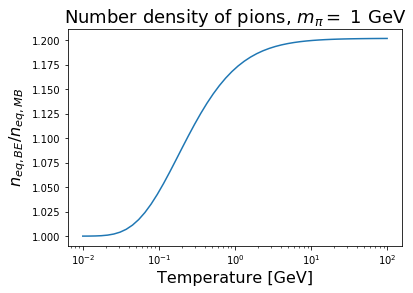
\includegraphics[width=0.45\textwidth]{bose.png}
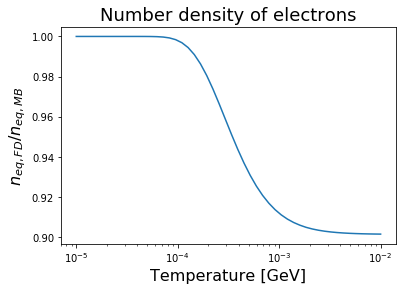
\includegraphics[width=0.45\textwidth]{pauli.png}
\caption{Bose enhancement and Pauli blocking.}
\end{figure}
Some example code for this would be 
\begin{lstlisting}[language=Python]
from particle_class import particle
import numpy as np
MBlist=[] 
FDlist=[]
#define ``classical'' and quantum electrons
MBelectron = particle(5e-4, 0.5, 2, 0.1, fast=True)
electron = particle(5e-4, 0.5, 2, 0.1)
#scan over temperatures
for i in np.logspace(-5, -2):
	#update temperatures and save eq number densities
	MBelectron.update(i), electron.update(i)
	MBlist.append(MBelectron.neq()), FDlist.append(electron.neq())
\end{lstlisting}

\section{Amplitudes}
The \code{amplitude} class essentially exists to take an amplitude do preprocessing for the \code{process} class. Essentially, you feed in a function and specify what type of amplitude it is (s-channel, three-point, WZW, etc.) and it can output part of the integrand for the thermally-averaged cross section. The main function of this class is \code{unweightedintegrand} which takes the arguments s (for the Mandelstam variable $s$), three energies, and four masses. Obviously the way it's written does not accommodate a five-point interaction so there is a specialized \code{WZWintegral} for that. Depending on the interaction type, different outputs are returned which correspond to the integrands (unweighted by DFs) which get numerically integrated over to give the collision term.
\subsection{Decays and Inverse Decays}
If the option \code{threept=True} is used, it is assumed that the pre-processing is being done for a decay or inverse decay. In this case the collision term takes the form 
\begin{align}
C = &\int \frac{\dbar^3 p_1}{2 E_1}\frac{\dbar^3 p_2}{2 E_2}\frac{\dbar^3 p_3}{2 E_3} f(E_1) (f(E_2)\pm1) (f(E_3)\pm1) (2 \pi)^4 \delta^{(4)}(p_1-p_2-p_3) \abs{\mathcal{M}}^2 \\
%=&2 \pi \int \frac{\dbar^3 p_1}{2 E_1}\frac{\dbar^3 p_2}{2 E_2} f(E_1) (f(E_2)\pm1) \left[\frac{1}{2 E_3}(f(E_3)\pm1) \delta(E_1-E_2-E_3) \abs{\mathcal{M}}^2\right]_{\vec{p}_3 = \vec{p}_1 - \vec{p}_2}\\
=&\frac{1}{2 \pi} \int \left[ \frac{\dbar^3 p_1 d x\, p_2^2 d p_2 }{8 E_1 E_2 E_3}f(E_1) (f(E_2)\pm1) (f(E_3)\pm1) \delta\left(E_1 - E_2 - E_3\right) \abs{\mathcal{M}}^2\right]_{E_3 = \sqrt{m_3^2 + p_1^2 + p_2^2 - 2 p_1 p_2 x}} \\
%=&\frac{1}{2 \pi} \int \left[ \frac{\dbar^3 p_1 d x\, p_2^2 d p_2 }{8 E_1 E_2 E_3}f(E_1) (f(E_2)\pm1) (f(E_3)\pm1) \frac{E_3}{p_1 p_2} \delta(x-x_0) \abs{\mathcal{M}}^2\right]_{E_3 = \sqrt{m_3^2 + p_1^2 + p_2^2 - 2 p_1 p_2 x}}\\%\\ x_0 = (m_3^2 + p_1^2 + p_2^2 - (E_2-E_1)^2)/2 p_1 p_2} \\
=&\frac{1}{4(2 \pi)^3} \int  \frac{p_1 d p_1 d x\, p_2 d p_2 }{ E_1 E_2}f(E_1) (f(E_2)\pm1) \delta(x-x_0)\left[ (f(E_3)\pm1)  \abs{\mathcal{M}}^2\right]_{E_3 = \sqrt{m_3^2 + p_1^2 + p_2^2 - 2 p_1 p_2 x}}\\
%=&\frac{1}{4(2 \pi)^3} \int \left[ \frac{ p_1 d p_1 p_2 d p_2 }{E_1 E_2}f(E_1) (f(E_2)\pm1) (f(E_3)\pm1) \abs{\mathcal{M}}^2\right]_{E_3 = \sqrt{m_3^2 + p_1^2 + p_2^2 - 2 p_1 p_2 x}, ~x = x_0} \\
=&\frac{1}{4(2 \pi)^3} \int  d E_1 d E_2 f(E_1) (f(E_2)\pm1)\left[ (f(E_3)\pm1) \abs{\mathcal{M}}^2\right]_{E_3 = \sqrt{m_3^2 + p_1^2 + p_2^2 - 2 p_1 p_2 x}, ~x = x_0}
\end{align}
where the factors of $f\pm 1$ account for BE/FD statistics, $x$ is introduced to track the cosine of the angle between $\vec{p}_1$ and $\vec{p}_2$, and $x_0  = (m_3^2 +p_1^2 + p_2^2  - (E_1-E_2)^2)/2 p_1 p_2$. Note that if we want the energy-weighted collision term, the steps above hold because nowhere did we evaluate things in any particular frame, we just have to add a factor of $E_1$ to the integrand of the final result.

Given the arguments above, the appropriate inputs for initializing an instance of the \code{amplitude} class are $\abs{\mathcal{M}}^2$ evaluated at $\vec{p}_3 = \vec{p}_1 - \vec{p}_2$ and $x=x_0$ along with the keyword argument \code{threept=True}. Then the function \code{unweightedintegrand} will then run through the following steps to process the parts of the integrand that don't involve distribution functions:
\begin{lstlisting}[language=Python]
#make sure there's enough energy budgeted to create third particle
if e2<e1-m3:
	p1 = p(e1,m1)
	p2 = p(e2,m2)
	#ensure cos of angle between final state particles is between -1 and 1
	x0 = (-(e2-e1)**2 + m3**2 + p1**2 +p2**2)/(2*p1*p2)
	if x0>-1 and x0<1:
		#return appropriately normalized unweighted integrand
		return 1/(4*(2*np.pi)**3)*self.form(s)
	else:
		return 0
else:
	return 0
\end{lstlisting}
The first criterion makes sure that we don't integrate over regions where there isn't enough energy left to account for $m_3$. The second criterion makes sure that a solution exists where the cosine between $\vec{p}_1$ and $\vec{p}_2$ is between -1 and 1. Both these criteria were implicitly imposed on the bounds of the integrals above upon evaluation of the delta functions.

The above also works for inverse decays, with the labels (or their interpretations) appropriately reshuffled.
\subsection{2$\,\rightarrow\,$2 Scattering and Annihilation}
So far, I've only coded up scattering for amplitudes that only depend on $s$ (or are trivial) following Appendix A of Adshead et al. (2016). The way to use this option is by setting \code{s=True}. It may be the case that for our purposes $t$ channel or more complicated functions of Mandelstam variables will be necessary, and thus I have the placeholder options \code{t} and \code{complicatedMandelstam}. Based on Adshead et al., the $t$ channel should be very straightforward, while something more complicated might require more care.

For $s$ channel (and trivial) processes, the key equation for our purposes is 
\beq C = \frac{\pi}{8 (2 \pi)^6} \int \frac{d E_1 d E_2 d E_3 ds}{\sqrt{(E_1+E_2)^2 - s}} \Theta(A) \Lambda(f_1, f_2, f_3, f_4) \hat{S} \abs{\mathcal{M}}^2 \eeq
where $\Lambda$ is the combination of distribution functions appearing for a specific collision term, $\hat{S}$ is a factor which includes symmetrization and counting of degrees of freedom, and the argument of the Heaviside function is 
\beq 
A = \frac{\left( \tilde{s} + (p_1 + p_2)^2\right)\left( \tilde{s} + (p_3 + p_4)^2\right)\left( \tilde{s} + (p_1 - p_2)^2\right)\left( \tilde{s} + (p_3 - p_4)^2\right)}{16 p_1^4 p_2^4 p_3^4}
\eeq
where $\tilde{s} \equiv s - (E_1 + E_2)^2$ and $p_4 = \sqrt{(E_1 + E_2 - E_3)^2 - m_4^2}$. Note that since, by definition, $s = (E_1+E_2)^2 - (\vec{p}_1 + \vec{p}_2)^2$, $\tilde{s}$ is restricted to \beq -(p_1 + p_2)^2 <\tilde{s} <-(p_1 - p_2)^2 \label{condition1}\eeq which means that for the Heaviside function to be nonzero we require 
\beq 
 -(p_3 + p_4)^2 <\tilde{s} <-(p_3 - p_4)^2. \label{condition2} \eeq
Therefore, the function \code{unweightedintegrand} will run through the following steps to return the parts of the integrand that don't include the distribution functions:
\begin{lstlisting}[language=Python]
#define s tilde
st = s - (e1 + e2)**2
#s tilde should be negative by definition
if st<0:   
	p1 = p(e1,m1)
	p2 = p(e2,m2)
	p3 = p(e3,m3)
	#ensure enough energy to create 4th particle
	if e1+e2-e3>m4:
		#define p4
		pf = np.sqrt((e1+e2-e3)**2 -m4**2)
		#check that cos between p1 and p2 is between -1 and 1
		if st+(p1+p2)**2>0 and st+(p1-p2)**2<0:
			#satisfy theta fct
			if st+(p3+pf)**2>0 and st+(p3-pf)**2<0:
				#return normalized unweighted integrand
				return np.pi/(8*(2*np.pi**6))*self.form(s)/math.sqrt((e1+e2)**2-s)
			else:
				return 0.0
		else:
			return 0.0
	else:
		return 0.0   
else:
	return 0.0
\end{lstlisting}
The first criterion ensures mathematical consistency of the definition of $\tilde{s}$. The second ensures that there is enough available energy to create the 4th particle. The next two criteria are just the conditions of \eqref{condition1} and \eqref{condition2}. If you follow the derivation of Adshead et al., there is no assumption of a particular frame so again weighting this by energy to get the energy-weighted collision term is a perfectly valid thing to do.
\subsection{Five Point Interactions}
Currently my code does not agree with the scalings presented in previous SIMP papers, and I'm not sure if the problem is at the \code{amplitude} stage or the \code{process} stage. Therefore I will postpone writing about this until I figure out what's going on.

\section{Processes}
\label{process_sec}
The chief purpose of the \code{process} class is to compute thermally-averaged cross sections (energy-weighted and otherwise)
either using Monte Carlo integration or optionally using analytic expressions by setting the keyword argument \code{analytic=True}. To initialize a member of the process class, you need to input which particles are in the intial and final states of the process (up to three particles can be accommodated), whether that process is transferring energy (the default is \code{nonequilibrium=False}) and other optional arguments that sets the limits of integration and number of points in the Monte Carlo. For example, suppose I wanted to look at elastic scattering (via a trivial amplitude) for keeping the pions and ALPs kinetically coupled. Then I would initialize that process as follows 
\begin{lstlisting}[language=Python]
pion = particle(1, 0, 5, 0.1)
alp = particle(0.2, 0, 1, 0.1)
#generate trivial amplitude
fourpt = amplitude(lambda s:1e-10, s=True)
#generate pi a --> pi a process with energy transfer
transfer = process(fourpt, i1=pion,i2=alp,f1=pion,f2=alp,nonequilibrium=True)
\end{lstlisting}
I can also look at ALP decay to photons, which following the rules above (evaluating the amplitude for decays with the proper values of $x_0$ etc) has $\abs{\mathcal{M}}^2 = 16 (p_2\cdot p_3)^2 / f^2 = 4 m_a^4/f^2$
\begin{lstlisting}[language=Python]
photon = particle(0, 1, 2, 0.1)
#generate amplitude (with proper evaluation at x = x0 etc)
alpPhotons = amplitude(lambda s: 4*alp.mass**4 *1e-10,threept=True)
#generate a --> gamma gamma process
decaytophotons = process(alpPhotons, i1=alp,f1=photon,f2=photon)
\end{lstlisting}
Based on the input particles, the class automatically parses what kind of process it is and thus knows how to integrate accordingly.

The main function acting on members of this class is \code{CrossSection}. If \code{analytic=True} is specified, the analytic expression (if known) will be evaluated at the relevant masses and temperatures. These analytic expressions are encoded in the  \code{analytics} class. Otherwise the cross section is computed using the \code{vegas} adaptive Monte Carlo integration algorithm. For a decay like ALPs to photons, the code for doing this looks like 
\begin{lstlisting}[language=Python]
if self.ptype == 'decay':
	#product of distribution functions (including terms for FD/BE statistics)
	self.BF = lambda ea,e1:self.i1.DF(ea)*self.f1.DFpm1(e1)*self.f2.DFpm1(ea-e1)
	#don't want energy weighting
	if self.nonequilibrium is False:
		#generate full integrand including DFs
		self.integrand = lambda e1,ea:self.BF(ea,e1)*\
		self.amplitude.unweightedintegrand(0,ea,0,e1,self.i1.mass,\
		self.f1.mass,self.f2.mass,0)
		#define integrator within energy boundaries
		decayintegrator = vegas.Integrator([[self.f1.mass,self.upperenergy],[self.i1.mass,self.upperenergy]])
		#train adaptive integration on some MC attempts
		decayintegrator(lambda x:self.integrand(x[0],x[1]),nitn=10,neval=self.nevals)
		#now that mesh is trained, start aggregating statistics
		result = decayintegrator(lambda x:self.integrand(x[0],x[1]),nitn=10,neval=self.nevals)
		return result 
\end{lstlisting}
Meanwhile, the code for computing the energy-weighted cross section for ALP-pion elastic scattering looks like this:
\begin{lstlisting}[language=Python]
if self.ptype == '2 to 2':
	#product of distribution functions (including terms for FD/BE statistics)
	self.BF = lambda e1,e2,e3: self.i1.DF(e1)*self.i2.DF(e2)*self.f1.DFpm1(e3)*self.f2.DFpm1(e1+e2-e3)
	#include energy weighting
	if self.nonequilibrium:
		#generate full integrand including DFs *and* Delta E
		self.integrand = lambda s,e1,e2,e3: self.BF(e1,e2,e3)*(e1-e3)\
		*self.amplitude.unweightedintegrand(s,e1,e2,e3,self.i1.mass,self.i2.mass,\
		self.f1.mass,self.f2.mass)
		#define integrator within energy boundaries
		sIntegrator = vegas.Integrator([[(self.i1.mass+self.i2.mass)**2,4*self.upperenergy**2],[self.i1.mass,self.upperenergy],[self.i2.mass,self.upperenergy],[self.f1.mass,self.upperenergy]])
		#train adaptive integration on some MC attempts
		sIntegrator(lambda x:self.integrand(x[0],x[1],x[2],x[3]),nitn=10, neval=self.nevals)
		#now that mesh is trained, start aggregating statistics
		result =sIntegrator(lambda x:self.integrand(x[0],x[1],x[2],x[3]),nitn=10, neval=self.nevals)
		return result
\end{lstlisting}
where the key differences are that there are more variables to integrate over (2 vs 4), the different form of the unweighted integrand (as set up by the \code{amplitudes} class) and the inclusion of the $E_1 - E_3$ factor to take into account that we want to look at the average energy gained or lost by one of the species of particles participating. Note for this to be correct, the ordering of the particles in the initial and final states as input into the code must be consistent.
\ks{talk about weird case of energy transfer for annihilations}

In the following subsections, I will demonstrate the use of the code using several examples and will also verify its agreement with analytic expressions (derived using MB statistics) in the appropriate low-temperature regime.

\subsection{ALPs Decaying to Photons}
After importing the relevant modules, the code that is needed is 
\begin{lstlisting}[language=Python]
alp=particle(0.5, 0, 1, 0.1)
photon=particle(0, 1, 2, 0.1)
#set lambda=1/f = 1e-5
alpPhotons=amplitude(lambda s: alp.mass**4*4e-10,threept=True)
#define process
decaytophotons=process(alpPhotons,i1=alp,f1=photon,f2=photon,nevals=3e3)
#also define analogous process using analytic expressions
decaytophotons_check=process(alpPhotons,i1=alp,f1=photon,f2=photon,analytic=True)
\end{lstlisting}
As a reminder, our expression for the cross section is 
\beq \left<\sigma v\right> = \frac{m_a^5\, T}{(2 \pi)^3\, n^a_{eq}} K_1(m_a/T)\eeq
Then, we may use this code to see what the thermally-averaged cross sections are for this process at various temperatures and for various ALP masses:
\begin{lstlisting}[language=Python]
#temperature values to scan over
tempscan = np.logspace(1, -2., 31)
#add a MB alp for consistency
MBalp = particle(0.5, 0, 1, 0.1, fast=True)

#start at 0.5 GeV
alp.mass_update(0.5)
MBalp.mass_update(0.5)
xsection=[]
approxxsection = []
for i in tempscan:
    alp.update(i)
    photon.update(i)
    MBalp.update(i)
    xsection.append(decaytophotons.CrossSection().val/alp.neq())
    approxxsection.append(1e-10*decaytophotons_check.CrossSection()/MBalp.neq())
    
#switch to mass of 0.1 GeV    
alp.mass_update(0.1)
MBalp.mass_update(0.1)
xsection2=[]
approxxsection2 = []
for i in tempscan:
    alp.update(i)
    photon.update(i)
    MBalp.update(i)
    #effectively lower coupling by factor of \sim 3
    xsection2.append(3e-1*decaytophotons.CrossSection().val/alp.neq())
    approxxsection2.append(3e-11*decaytophotons_check.CrossSection()/MBalp.neq())
\end{lstlisting}
 \begin{figure}[h!]
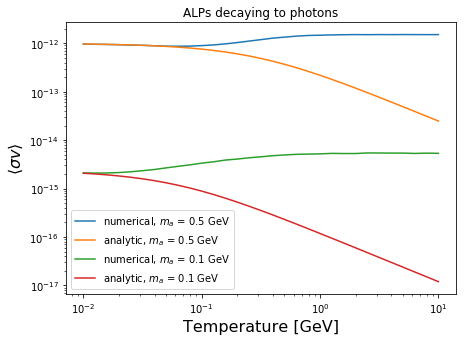
\includegraphics[width=0.65\textwidth]{alpdecay.png}
\caption{Comparison between the analytic expression and the full numerical integration for different masses, temperatures, and couplings. They agree well at low temperatures ($T\sim m/5$), where the particles are kinematically restricted to be on the MB tails of their distributions.}
\label{alpphoton}
\end{figure}

From these runs, it is clear that while the analytics and numerics agree at low temperatures, they do not agree at high temperatures. One might think that this could come from a lack of convergence. To test the discrepancy in the high temperature regime, the code has some optional inputs. One option is to check convergence of the MC integration by increasing the number of points with the optional \code{nevals} argument:
\begin{lstlisting}[language=Python]
decaytophotons = process(alpPhotons,i1=alp,f1=photon,f2=photon,nevals=3e3)
highres_decay = process(alpPhotons,i1=alp,f1=photon,f2=photon,nevals=1e4)
higherres_decay = process(alpPhotons,i1=alp,f1=photon,f2=photon,nevals=3e4)
\end{lstlisting}
Running the code above at high temperatures shows that the MC has indeed converged to within 5\%. Another culprit may be the cutoff in the energy, which is controlled by the optional \code{Ecut} parameter, which is 5 by default. This can be changed to test the effects of this energy cutoff as follows
\begin{lstlisting}[language=Python]
decaytophotons_highE=process(alpPhotons,i1=alp,f1=photon,f2=photon,nevals=1e4,Ecut=10)
decaytophotons_higherE=process(alpPhotons,i1=alp,f1=photon,f2=photon,nevals=1e4,Ecut=20)
\end{lstlisting}
Running the above at high temperatures again shows convergence, this time at the percent level. I am left to conclude that this discrepancy is physical and comes from the inclusion of $1+f$ terms which manifests as Bose enhancement.
\subsection{ALPs decaying to electrons}
Following the exact same steps above, except with decay to electrons, we can once again compare the numerics to the analytic expressions. In the code, we simply add 
\begin{lstlisting}[language=Python]
#create electrons
electron = particle(5e-4, 1/2, 2, 0.1)
alpElectrons = amplitude(lambda s:2*alp.mass**2*electron.mass**2,threept=True)
decaytoelectrons=process(alpElectrons,i1=alp,f1=electron,f2=electron,nevals=3e3)
decaytoelectrons_check=process(alpElectrons, i1=alp,f1=electron,f2=electron, analytic=True)
\end{lstlisting}
 \begin{figure}[h!]
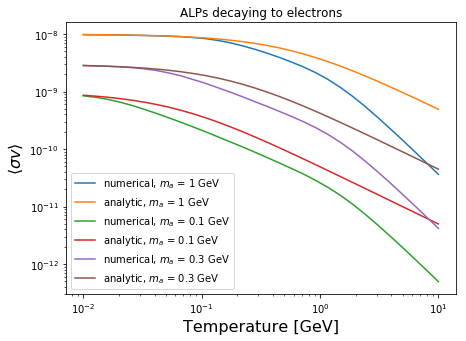
\includegraphics[width=0.65\textwidth]{electrondecay.png}
\caption{Same as Fig.~\ref{alpphoton} but with decay to electrons.}
\end{figure}
where, recall that $\abs{\mathcal{M}}^2  = 4 m_e^2 (p_2\cdot p_3 + m_e^2)/f^2$ and imposing the delta functions sets $\abs{\mathcal{M}}^2 \rightarrow 2 m_e^2 m_a^2/f^2$. The analytic expression to compare with is \beq \langle \sigma v \rangle =  \frac{m_a^2 m_e^2 \sqrt{m_a^4/4 - m_e^2}~ T}{(2 \pi)^3 \,n^a_{eq}} K_1(m_a/T).\eeq

As with the decay to photons, the high-temperature behavior for the decay to electrons differs between our analytic approximations and the numerics. The key difference is that the numerics fall below (rather than above) the analytic estimates, and differ by a smaller amount than for the decay to photons; this is consistent with my assertion that this difference arises due to spin statistics, as the numerical effects of Pauli blocking are smaller than for Bose enhancement. Checking the numerics as above, I find that this difference cannot be accounted for by a lack of convergence of my integrals.
\subsection{Pions Annihilating to ALPs}
In analogy to the examples above, the relevant code to add for looking at pion annihilation to ALPs is 
\begin{lstlisting}[language=Python]
#initialize pions and alps
pion = particle(1, 0, 5, 0.1)
alp = particle(0.5, 0, 1, 0.1)
#trivial amplitude
fourpt = amplitude(lambda s:1e-10, s=True)
#more MC points are necessary since the integral is higher dimensional
annihilation=process(fourpt, i1=pion,i2=pion,f1=alp,f2=alp,nevals=3e4)
\end{lstlisting}
and the analytic expression to compare to is 
\beq 
\langle \sigma v \rangle = \frac{T}{16 (2 \pi)^5} \int_{4 m_\pi^2}^{\infty} ds\, \sqrt{s} \,\lambda^{1/2}(\sqrt{s}, m_\pi, m_\pi)\lambda^{1/2}(\sqrt{s}, m_a, m_a) K_1 (\sqrt{s}/T)
\eeq
where $\lambda(x, y, z) \equiv (1 - (y + z)^2/x^2) (1 - (y- z)^2/x^2)$.
%#temperatures to integrate over
%tempscan = np.logspace(1, -1.5, 10)
%#MB version of a pion in order to do consistent between MB and full BE stats
%MBpion = particle(1, 0, 5, 0.1, fast=True)

%#look at these values of the mass
%alp.mass_update(0.5)
%pion.mass_update(1), MBpion.mass_update(1)
%xsection=[]
%approxxsection = []
%for i in tempscan:
%    alp.update(i), pion.update(i), MBpion.update(i)
%    xsection.append(annihilation.CrossSection().val/pion.neq()**2)
%    approxxsection.append(1e-10*annihilation_check.CrossSection()/MBpion.neq()**2)
%    
%#now look at different masses
%alp.mass_update(0.2)
%pion.mass_update(0.7),MBpion.mass_update(0.7)
%xsection2=[]
%approxxsection2 = []
%for i in tempscan:
%    alp.update(i), pion.update(i),MBpion.update(i)
%    #effectively change coupling
%    xsection2.append(3e-1*annihilation.CrossSection().val/pion.neq()**2)
%    approxxsection2.append(3e-11*annihilation_check.CrossSection()/MBpion.neq()**2)

 \begin{figure}[h!]
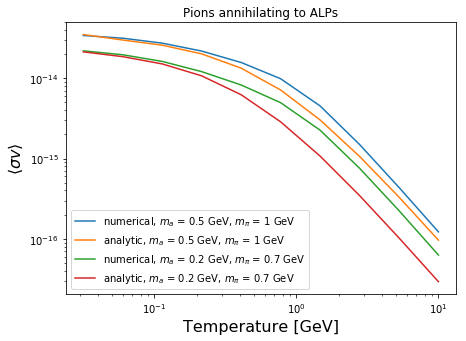
\includegraphics[width=0.65\textwidth]{annihilation.png}
\caption{Same as Fig.~\ref{alpphoton} but for pions annihilating into ALPs. Note: the normalizations have been adjusted in this figure to be consistent, as they appear to be off from each other by a factor of $\sim(2 \pi)^2$.}
\end{figure}
As with above, the two curves disagree at high temperatures. Here because the particles involved are bosons, the numerics give an answer that is larger than the analytics. Again going through the exercise of checking convergence, we find that the discrepancy cannot be accounted for by anything other than Bose enhancement.

\subsection{The Effects of Different Temperatures}
It's important to point out that in the analytic expressions, only one temperature is used because the $f\pm1$ terms are set to 1 and therefore according to those expressions the cross section should only be a function of the temperature of the initial state particle. However, using full numerics it's easy to see that this is not the case and this can affect both the thermal shape and normalizations of the cross sections.
 \begin{figure}[h!]
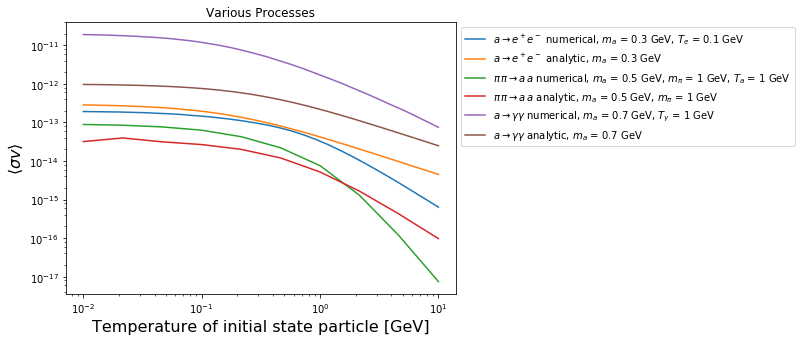
\includegraphics[width=\textwidth]{difftemp.png}
\caption{Comparison between analytics and numerics for a variety of processes. Here we have set the final state particle to have a fixed temperature. According to the analytic approximations, this should have no effect on the answer; however, we see that in fixing the temperature of the final particles, the analytics and numerics no longer track.}
\end{figure}

\section{Solving the Boltzmann Equations}
\subsection{Implicit Methods for Stiff Systems of Equations}
This discussion basically summarizes the analogous sections in Numerical Recipes by Press, Teukolsky, et al. about stiff systems. The key pathology which makes these systems difficult to evaluate numerically is that even with linear differential equations, there can be huge discrepancies in the timescales required to resolve the evolution. In our case, there is a very physical way to see the disparity of timescales: we want to resolve particle collisions, which at early times (before freezeout) happen very fast relative to the Hubble time on average. The simpler example given in NR is \beq u' = 998 u +1998 v \quad \quad \quad v' = -999 u - 1999 v \eeq with boundary conditions $u(0) = 1$ and $v(0) = 0$.
This has the solution \beq u = 2 e^{-x} - e^{-1000 x} \quad \quad \quad v = - e^{-x} + e^{-1000 x} .\eeq Analytically speaking, the second term is completely negligible away from the origin. However, in general numerical methods have a hard time realizing this unless the stepsize is small enough (roughly 1000$\times$ smaller than if the second term were not present) and in general the numerical evolution will have severe instabilities. To see this, consider the following simplified example: \beq y' = -c y \quad \Rightarrow \quad y_{n+1} = y_n + h y'_n = (1 - c h ) y_n.\eeq
By forward evolving in this way, we can see that this method is unstable because if $h>2/c$ then $\abs{y_n} \rightarrow \infty$ as $n\rightarrow \infty$. Even though this is a simplified example using Euler's method, any forward evolution scheme will suffer from the same pathology (including RK and other higher order methods). The simplest cure is to use backward evolution \beq y_{n+1} = y_n + h y'_{n+1} \Rightarrow y_{n+1} = y_n / (1 + c h )\eeq which damps out any runaway oscillations and converges as $n\rightarrow \infty$.

To generalize this to a nonlinear system of differential equations, we can try linearizing the equations in an analogous way and find a matrix equation of the form \beq \vec{y}' = \vec{f}(\vec{y}) \quad \Rightarrow \quad  \vec{y}_{n+1}  = \vec{y}_n + h \left[ \mathbbold{1} - h \frac{\partial\vec{f} }{\partial \vec{y}} \right]^{-1} \cdot \vec{f}(\vec{y}_n) \label{implicit} \eeq
where $\partial \vec{f} /\partial \vec{y}$ is the Jacobian matrix. This is the semi-implicit backwards Euler method, and while it is not guaranteed to be stable, it will be stable for small enough step size because it is locally similar to the linear constant coefficient case.
\subsection{Stable Variable Choice}
The raw form of the Boltzmann equations (from integrating over the equation for phase space density evolution)  is \beq \dot{n}_X + 3 H n_X = \sum_i C_i \left(\frac{n_{Y, i}}{n^{eq}_{Y, i}}  \right)^{k_i} \quad \quad \dot{\rho} + 3 H (p + \rho) = \sum_i C_i' \left(\frac{n_{Y, i}}{n^{eq}_{Y, i}}  \right)^{k_i}\eeq
where $X$ is some species, dots denote derivatives with respect to time, and the sum is over collision terms involving any species that interact with $X$ through scattering, decay etc. (the type of interaction is captured by the exponent $k$). Note the collision factor $C$ and $C'$ (the energy-weighted version of $C$) are different from $\langle\sigma v\rangle$ because they do not contain any factors of $n^{eq}$ in the denominator. I will use $a$ as my time coordinate as opposed to $t$ or $T$ (which is a common choice) because here we do not \emph{a priori} know $T(a)$, unlike for the WIMP case where $T \sim 1/a$. 

In addition to the implicit methods described above, another way to ensure stability is to parameterize the solution as a deviation away from some function, which need not be explicitly known. For the equation parametrizing the number density, I use $ u  = n / n_{eq} - 1$ while for the equation parametrizing the energy density I use $ v= a T - 1$. With these choices of variables, the Boltzmann equations become 
\begin{align}
&\frac{d u_X }{d a} = -\frac{(u_X+1)}{n^{eq}_X} \frac{d n^{eq}_X}{d T_X}\frac{dT_X }{d a} - \frac{3 (u_X + 1)}{a} + \frac{1}{a H(a) n^{eq}_X} \sum_i C_i (u_{Y, i} + 1)^{k_i}\label{ueqn}\\
&\frac{d v_X }{d a} =\frac{v_X+1}{a} + \frac{1}{d \rho_X /d T_X} \left( -3 (\rho_X + p_X) + \sum_i C_i (u_{Y, i} + 1)^{k_i} / H(a)\right). \label{veqn}
\end{align}
Since we are deep in the radiation-dominated regime, we will (for the time being) assume a constant number of relativistic degrees of freedom and use \beq H^2 = \frac{8 \pi G}{3}\frac{\pi^2 g_*}{30} T^4 \Rightarrow H(a) = \frac{H(T = \text{1 GeV})}{ a^2}.\eeq 
Some of the derivatives coming from the Jacobian of our variable transformation can be determined analytically if the forms \eqref{neq}-\eqref{peq} are assumed, for instance $d n^{eq}/d T$. The value of $d T_X/d a$ can be numerically determined from \eqref{veqn}.

In addition to the equations above, the Jacobian matrix for this system of ODEs is also necessary in order to time evolve. Not only would this be tricky to do analytically since the RHS of \eqref{ueqn}-\eqref{veqn} is complicated, but there are also hidden dependences on the variables in the collision terms. For instance, even for $s$-wave processes there is a nonzero dependence on temperature, as can be seen in the plots of Section~\ref{process_sec}. This $T$-dependence (and hence influence on the jacobian) could in principle be determined from analytic expressions for processes where those are available-- however since they are not available for all processes, and since they are not correct at higher temperatures, we will want some way to determine the jacobian numerically.
\subsection{Numerical Code}
With the above method and variable choice in mind, the \code{ode\_helper} script has several functions which compute the necessary ingredients for evolving the equations above. 

First off, to speed up the code the quantities $n^{eq}$, $\rho$, $p$ and their temperature derivatives are coded up using the expressions in \eqref{neq}-\eqref{peq} (rather than the full integrals, which take roughly ten times longer to evaluate than Bessel functions) as a function of temperature and chemical potential, which are in turn functions of $u$ and $v$. We emphasize that using MB statistics in evolving some terms in the code is a better approximation than using it for computing the thermally-averaged cross sections-- in the former case each term can be off by as much as 10\% whereas in the latter case it can change the result by orders of magnitude.
 
The main function is \code{derivatives} which computes the RHS of \eqref{ueqn}-\eqref{veqn} at every timestep. The mandatory inputs to \code{derivatives} are the scale factor $a$, a list of the pion and alp objects in the particle class (so that the function can access their attributes like temperature), and a list of the current values of $u$ and $v$ for each of the particles. Additionally, different processes can be turned on (their default is to be turned off) by passing the optional keyword arguments corresponding to each process. The inputs for these arguments should be of the form of an interpolating function (i.e. the lookup table you read in from the \code{.pkl} file) except in the case of the WZW term which should just be a number (since I still am using the analytic form for it and haven't figured out why the full integral doesn't work.) Currently, for simplicity, I have forward processes and backward processes having the same thermally-averaged cross section in the Boltzmann equation, but this is not necessary nor is it hard-coded in. Other optional arguments set the strength of the couplings between ALPs and pions/ ALPs and photons. Using these inputs, the function first computes the derivatives for $v$ and then this is used to compute the $d T/d a$ factor that appears in the derivatives for $u$. 

The final necessary piece is the jacobian, which is computed using the \code{numdifftools} package. Forward derivatives are computed, since the boundary conditions are $u = v = 0$ and dipping below 0 is unphysical and causes the code to crash.

In the ipython notebook, you have to specify a grid over which to integrate the Boltzmann equations. For now I'm using a linear grid, but this can be easily changed to accommodate more sensitive dynamics. I'm starting the evolution at $T=$1 GeV with the initial condition that $u= v= 0$. The code calls the derivative and jacobian functions and computes the next step using \eqref{implicit}. Before updating the values of $u$ and $v$, intermediate values of number density, temperature, and the derivatives (in particular the WZW term).
\end{document}